% ============================================================
%  FinSentNet — Model Design Diagrams (TikZ, paper-ready)
%  Compile on Overleaf (pdfLaTeX) or locally: pdflatex finsent_diagrams.tex
%  Every figure is wrapped in \resizebox so it never overflows the page.
% ============================================================
\documentclass[11pt]{article}
\usepackage[a4paper,margin=1.5cm,landscape]{geometry}
\usepackage{graphicx} % for \resizebox
\usepackage{tikz}
\usepackage{amsmath}
\usetikzlibrary{positioning,arrows.meta,calc,fit,backgrounds,shapes.geometric,shapes.misc}

% ---- Shared palette ----
\definecolor{cInput}{HTML}{455A64}
\definecolor{cText}{HTML}{1565C0}
\definecolor{cPrice}{HTML}{E65100}
\definecolor{cFusion}{HTML}{6A1B9A}
\definecolor{cOut}{HTML}{00838F}
\definecolor{cTrade}{HTML}{2E7D32}
\definecolor{cRisk}{HTML}{C62828}
\definecolor{cGan}{HTML}{AD1457}
\definecolor{cBg}{HTML}{ECEFF1}

% ---- Shared node styles ----
\tikzset{
  base/.style   ={rounded corners=2pt, draw, align=center, font=\small,
                  minimum height=8mm, inner sep=4pt, line width=0.5pt},
  io/.style     ={base, fill=cInput!12,  draw=cInput,  text=black},
  tnode/.style  ={base, fill=cText!12,   draw=cText,   text=black},
  pnode/.style  ={base, fill=cPrice!14,  draw=cPrice,  text=black},
  fnode/.style  ={base, fill=cFusion!12, draw=cFusion, text=black},
  onode/.style  ={base, fill=cOut!14,    draw=cOut,    text=black},
  trnode/.style ={base, fill=cTrade!12,  draw=cTrade,  text=black},
  rnode/.style  ={base, fill=cRisk!12,   draw=cRisk,   text=black},
  gnode/.style  ={base, fill=cGan!12,    draw=cGan,    text=black},
  group/.style  ={rounded corners=4pt, draw, dashed, line width=0.6pt, inner sep=6pt},
  arr/.style    ={-{Latex[length=2.2mm]}, line width=0.7pt},
  arrb/.style   ={{Latex[length=2.2mm]}-{Latex[length=2.2mm]}, line width=0.7pt},
  lbl/.style    ={font=\scriptsize\itshape, fill=white, inner sep=1pt},
}

\begin{document}
\pagestyle{empty}

% =====================================================================
% FIGURE 1 — WHOLE SYSTEM ARCHITECTURE
% =====================================================================
\begin{figure}[p]\centering
\resizebox{\textwidth}{!}{%
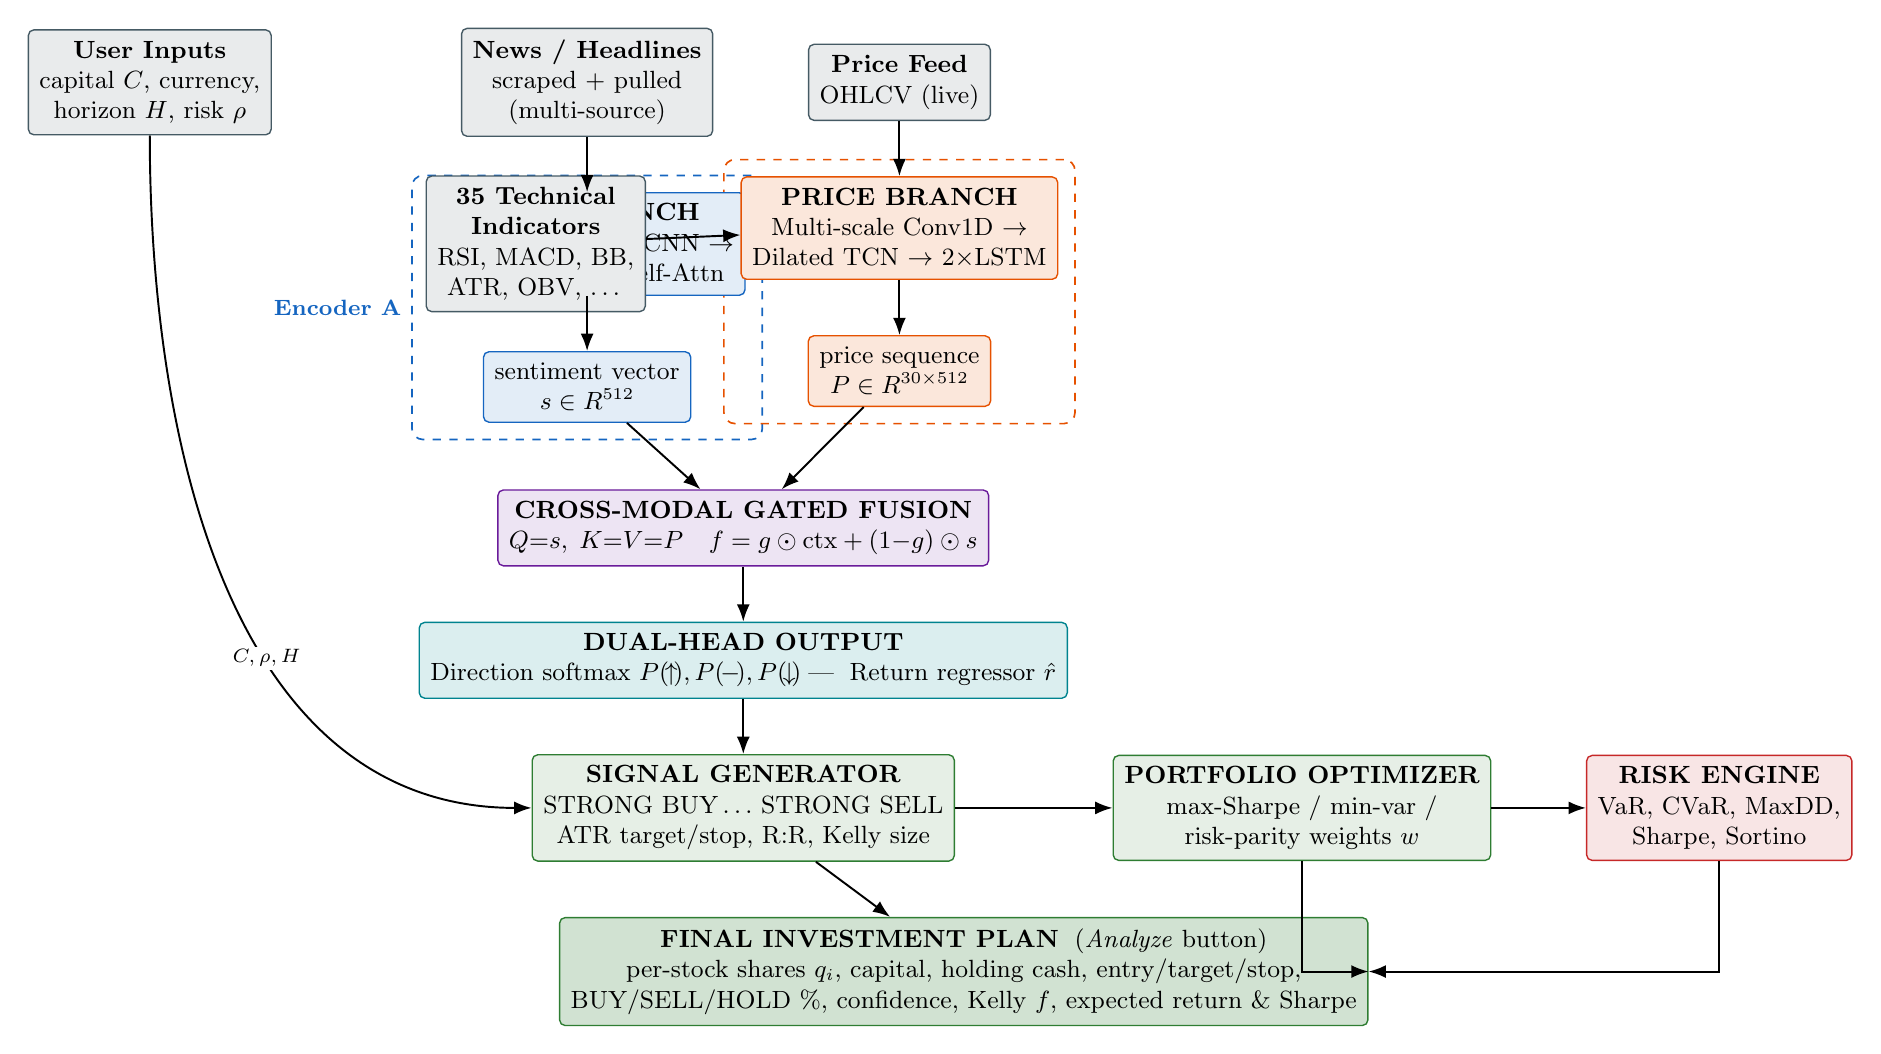
\begin{tikzpicture}[node distance=7mm and 12mm]

% --- Inputs ---
\node[io] (user)  {\textbf{User Inputs}\\ capital $C$, currency,\\ horizon $H$, risk $\rho$};
\node[io, right=24mm of user] (news) {\textbf{News / Headlines}\\ scraped + pulled\\ (multi-source)};
\node[io, right=12mm of news] (px)  {\textbf{Price Feed}\\ OHLCV (live)};

% --- Branches ---
\node[tnode, below=of news] (tb)
   {\textbf{TEXT BRANCH}\\ FinBERT $\to$ TextCNN $\to$\\ 3$\times$BiLSTM $\to$ Self-Attn};
\node[pnode, below=of px] (pb)
   {\textbf{PRICE BRANCH}\\ Multi-scale Conv1D $\to$\\ Dilated TCN $\to$ 2$\times$LSTM};
\node[io, left=12mm of pb, yshift=-2mm] (ti)
   {\textbf{35 Technical}\\ \textbf{Indicators}\\ RSI, MACD, BB,\\ ATR, OBV, \dots};

% --- Vectors ---
\node[tnode, below=of tb] (svec) {sentiment vector\\ $s \in \mathbb{R}^{512}$};
\node[pnode, below=of pb] (pvec) {price sequence\\ $P \in \mathbb{R}^{30\times512}$};

% --- Fusion ---
\node[fnode, below=14mm of $(svec)!0.5!(pvec)$] (fus)
   {\textbf{CROSS-MODAL GATED FUSION}\\
    $Q{=}s,\;K{=}V{=}P$\quad
    $f = g\odot\mathrm{ctx} + (1{-}g)\odot s$};

% --- Dual head ---
\node[onode, below=of fus] (dh)
   {\textbf{DUAL-HEAD OUTPUT}\\
    Direction softmax $P(\!\uparrow\!),P(\!-\!),P(\!\downarrow\!)$\;|\;
    Return regressor $\hat r$};

% --- Decision layer ---
\node[trnode, below=of dh] (sig)
   {\textbf{SIGNAL GENERATOR}\\ STRONG BUY\,$\dots$\,STRONG SELL\\
    ATR target/stop, R:R, Kelly size};
\node[trnode, right=20mm of sig] (port)
   {\textbf{PORTFOLIO OPTIMIZER}\\ max-Sharpe / min-var /\\ risk-parity weights $w$};
\node[rnode, right=12mm of port] (risk)
   {\textbf{RISK ENGINE}\\ VaR, CVaR, MaxDD,\\ Sharpe, Sortino};

% --- Output ---
\node[io, below=of sig, xshift=28mm, fill=cTrade!22, draw=cTrade] (plan)
   {\textbf{FINAL INVESTMENT PLAN} \;(\textit{Analyze} button)\\
    per-stock shares $q_i$, capital, holding cash, entry/target/stop,\\
    BUY/SELL/HOLD \%, confidence, Kelly $f$, expected return \& Sharpe};

% --- Edges ---
\draw[arr] (news) -- (tb);
\draw[arr] (px)   -- (pb);
\draw[arr] (ti)   -- (pb);
\draw[arr] (tb)   -- (svec);
\draw[arr] (pb)   -- (pvec);
\draw[arr] (svec) -- (fus);
\draw[arr] (pvec) -- (fus);
\draw[arr] (fus)  -- (dh);
\draw[arr] (dh)   -- (sig);
\draw[arr] (sig)  -- (port);
\draw[arr] (port) -- (risk);
\draw[arr] (sig)  -- (plan);
\draw[arr] (port) |- (plan);
\draw[arr] (risk) |- (plan);
% user params steer sizing
\draw[arr] (user.south) to[out=-90,in=180] node[lbl,pos=0.6]{$C,\rho,H$} (sig.west);

% --- Background groups ---
\begin{scope}[on background layer]
  \node[group, draw=cText,  fit=(tb)(svec), label={[cText,font=\footnotesize\bfseries]left:Encoder A}] {};
  \node[group, draw=cPrice, fit=(pb)(pvec)] {};
\end{scope}
\end{tikzpicture}}
\caption{FinSentNet end-to-end architecture: dual encoders $\to$ cross-modal gated fusion $\to$ dual-head $\to$ signal/portfolio/risk $\to$ final plan.}
\end{figure}

% =====================================================================
% FIGURE 2 — TEXT BRANCH (6 layers)
% =====================================================================
\begin{figure}[p]\centering
\resizebox{0.92\textwidth}{!}{%
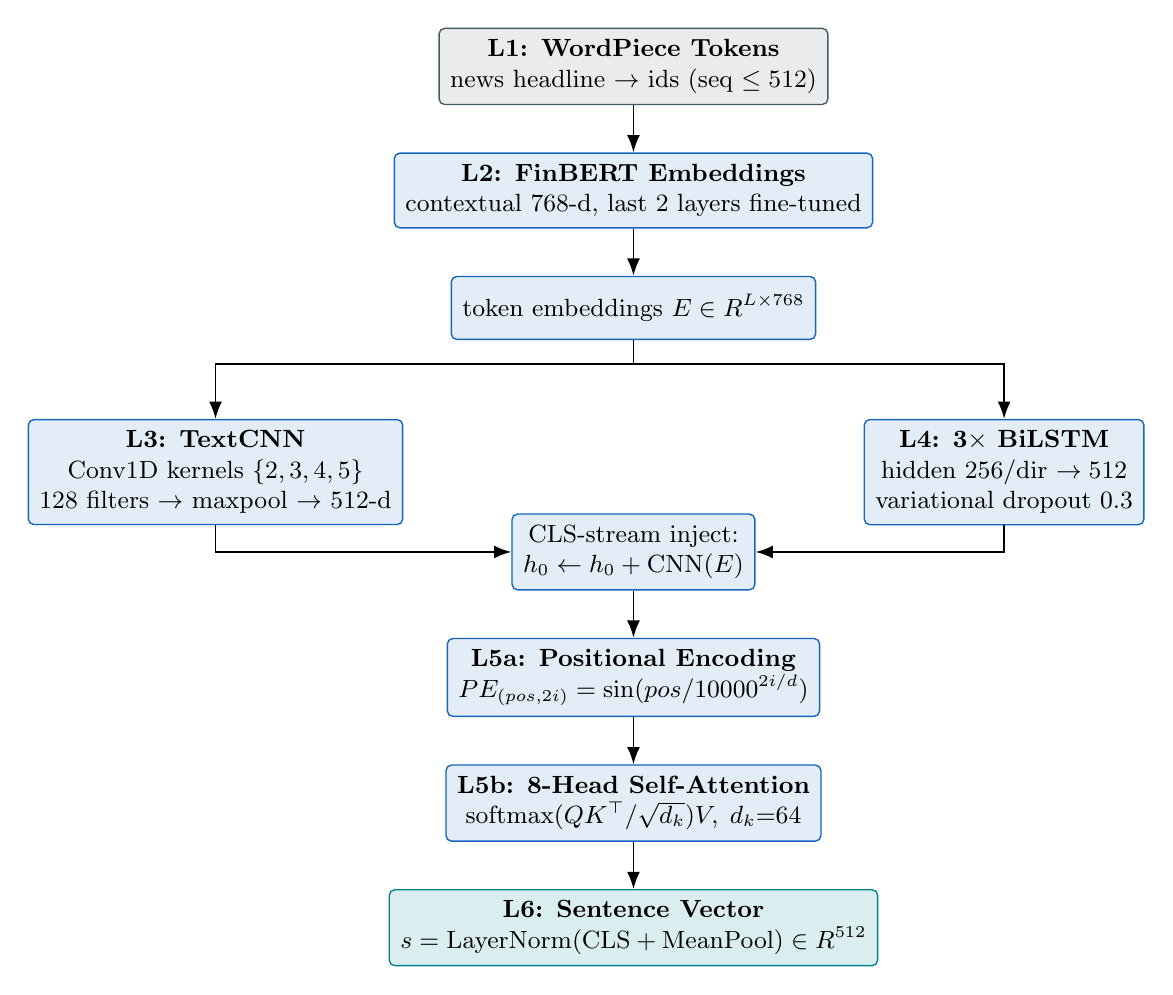
\begin{tikzpicture}[node distance=6mm]
\node[io] (tok) {\textbf{L1: WordPiece Tokens}\\ news headline $\to$ ids (seq $\le 512$)};
\node[tnode, below=of tok] (emb) {\textbf{L2: FinBERT Embeddings}\\ contextual $768$-d, last 2 layers fine-tuned};
\node[tnode, below=of emb] (split) {token embeddings $E\in\mathbb{R}^{L\times768}$};

\node[tnode, below left=10mm and 6mm of split] (cnn)
   {\textbf{L3: TextCNN}\\ Conv1D kernels $\{2,3,4,5\}$\\ 128 filters $\to$ maxpool $\to$ $512$-d};
\node[tnode, below right=10mm and 6mm of split] (lstm)
   {\textbf{L4: 3$\times$ BiLSTM}\\ hidden 256/dir $\to 512$\\ variational dropout 0.3};

\node[tnode, below=22mm of split] (inject) {CLS-stream inject:\\ $h_0 \leftarrow h_0 + \mathrm{CNN}(E)$};
\node[tnode, below=of inject] (pos) {\textbf{L5a: Positional Encoding}\\ $PE_{(pos,2i)}=\sin(pos/10000^{2i/d})$};
\node[tnode, below=of pos] (attn) {\textbf{L5b: 8-Head Self-Attention}\\ $\mathrm{softmax}(QK^\top/\sqrt{d_k})V,\;d_k{=}64$};
\node[onode, below=of attn] (pool)
   {\textbf{L6: Sentence Vector}\\ $s=\mathrm{LayerNorm}(\mathrm{CLS}+\mathrm{MeanPool})\in\mathbb{R}^{512}$};

\draw[arr] (tok)--(emb); \draw[arr] (emb)--(split);
\draw[arr] (split.south) -- ++(0,-3mm) -| (cnn.north);
\draw[arr] (split.south) -- ++(0,-3mm) -| (lstm.north);
\draw[arr] (cnn.south) |- (inject.west);
\draw[arr] (lstm.south) |- (inject.east);
\draw[arr] (inject)--(pos); \draw[arr] (pos)--(attn); \draw[arr] (attn)--(pool);
\end{tikzpicture}}
\caption{Text branch: 6-layer FinBERT $\to$ TextCNN $\to$ BiLSTM $\to$ self-attention sentiment encoder.}
\end{figure}

% =====================================================================
% FIGURE 3 — PRICE BRANCH (5 layers)
% =====================================================================
\begin{figure}[p]\centering
\resizebox{0.95\textwidth}{!}{%
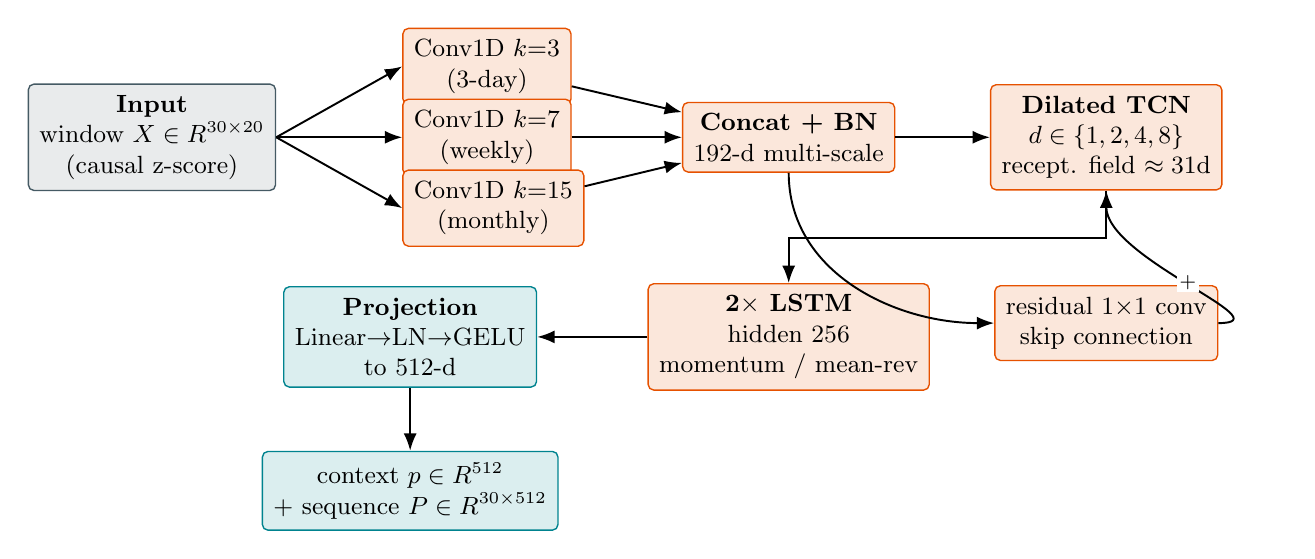
\begin{tikzpicture}[node distance=6mm and 10mm]
\node[io] (in) {\textbf{Input}\\ window $X\in\mathbb{R}^{30\times20}$\\ (causal z-score)};

\node[pnode, right=16mm of in, yshift=9mm]  (c3)  {Conv1D $k{=}3$\\ (3-day)};
\node[pnode, right=16mm of in]              (c7)  {Conv1D $k{=}7$\\ (weekly)};
\node[pnode, right=16mm of in, yshift=-9mm] (c15) {Conv1D $k{=}15$\\ (monthly)};
\node[pnode, right=14mm of c7] (cat) {\textbf{Concat + BN}\\ $192$-d multi-scale};

\node[pnode, right=12mm of cat] (dil)
   {\textbf{Dilated TCN}\\ $d\in\{1,2,4,8\}$\\ recept. field $\approx 31$d};
\node[pnode, below=12mm of dil] (res) {residual $1{\times}1$ conv\\ skip connection};

\node[pnode, below=14mm of cat] (lstm) {\textbf{2$\times$ LSTM}\\ hidden 256\\ momentum / mean-rev};
\node[onode, left=14mm of lstm] (proj)
   {\textbf{Projection}\\ Linear$\to$LN$\to$GELU\\ to $512$-d};
\node[onode, below=8mm of proj] (out)
   {context $p\in\mathbb{R}^{512}$\\ + sequence $P\in\mathbb{R}^{30\times512}$};

\draw[arr] (in.east) -- (c3.west);
\draw[arr] (in.east) -- (c7.west);
\draw[arr] (in.east) -- (c15.west);
\draw[arr] (c3) -- (cat); \draw[arr] (c7) -- (cat); \draw[arr] (c15) -- (cat);
\draw[arr] (cat) -- (dil);
\draw[arr] (cat.south) to[out=-90,in=180] (res.west);
\draw[arr] (res.east) to[out=0,in=-90] node[lbl]{$+$} (dil.south);
\draw[arr] (dil.south) -- ++(0,-6mm) -| (lstm.north);
\draw[arr] (lstm) -- (proj);
\draw[arr] (proj) -- (out);
\end{tikzpicture}}
\caption{Price branch: multi-scale Conv1D $\to$ dilated temporal CNN (residual) $\to$ LSTM $\to$ projected price context + sequence.}
\end{figure}

% =====================================================================
% FIGURE 4 — CROSS-MODAL GATED FUSION (core innovation)
% =====================================================================
\begin{figure}[p]\centering
\resizebox{0.9\textwidth}{!}{%
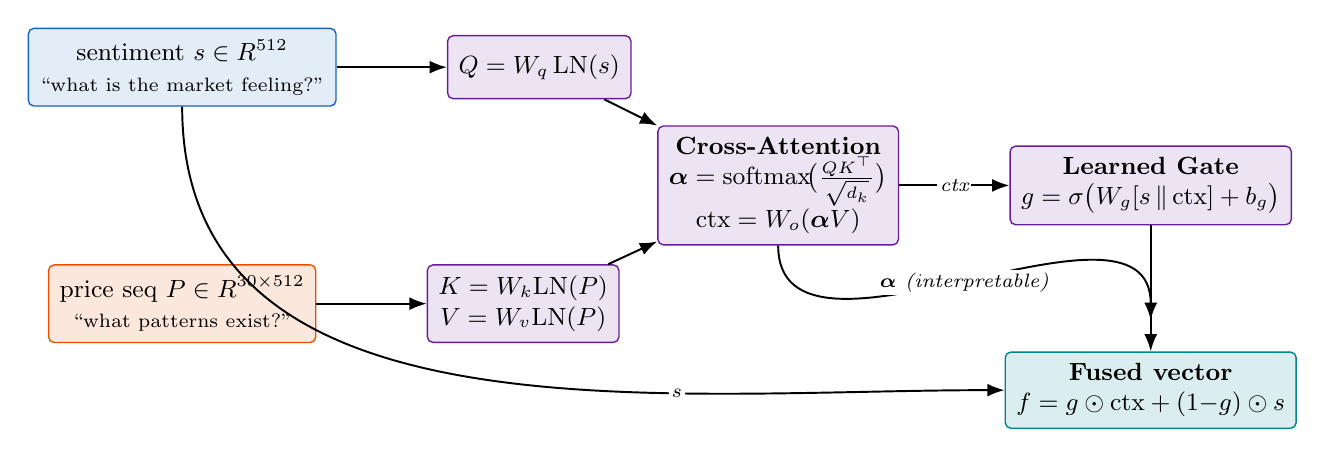
\begin{tikzpicture}[node distance=8mm and 14mm]
\node[tnode] (s) {sentiment $s\in\mathbb{R}^{512}$\\ \scriptsize``what is the market feeling?''};
\node[pnode, below=20mm of s] (P) {price seq $P\in\mathbb{R}^{30\times512}$\\ \scriptsize``what patterns exist?''};

\node[fnode, right=of s]  (q) {$Q=W_q\,\mathrm{LN}(s)$};
\node[fnode, right=of P]  (kv){$K=W_k\mathrm{LN}(P)$\\ $V=W_v\mathrm{LN}(P)$};

\node[fnode, right=16mm of $(q)!0.5!(kv)$] (att)
   {\textbf{Cross-Attention}\\
    $\boldsymbol\alpha=\mathrm{softmax}\!\big(\tfrac{QK^\top}{\sqrt{d_k}}\big)$\\
    $\mathrm{ctx}=W_o(\boldsymbol\alpha V)$};

\node[fnode, right=of att] (gate)
   {\textbf{Learned Gate}\\ $g=\sigma\big(W_g[s\,\Vert\,\mathrm{ctx}]+b_g\big)$};
\node[onode, below=16mm of gate] (fused)
   {\textbf{Fused vector}\\ $f=g\odot\mathrm{ctx}+(1{-}g)\odot s$};

\draw[arr] (s) -- (q);
\draw[arr] (P) -- (kv);
\draw[arr] (q)  -- (att);
\draw[arr] (kv) -- (att);
\draw[arr] (att) -- node[lbl]{ctx} (gate);
\draw[arr] (gate) -- (fused);
\draw[arr] (s.south) to[out=-90,in=180] node[lbl,pos=0.7]{$s$} (fused.west);
\draw[arr] (att.south) to[out=-90,in=90] node[lbl]{$\boldsymbol\alpha$ (interpretable)} ($(fused.north)+(0,4mm)$);
\end{tikzpicture}}
\caption{Cross-modal gated attention fusion: sentiment queries price history; a learned sigmoid gate adaptively blends modalities (sentiment-driven on news days, price-driven on breakouts).}
\end{figure}

% =====================================================================
% FIGURE 5 — DUAL-HEAD OUTPUT
% =====================================================================
\begin{figure}[p]\centering
\resizebox{0.78\textwidth}{!}{%
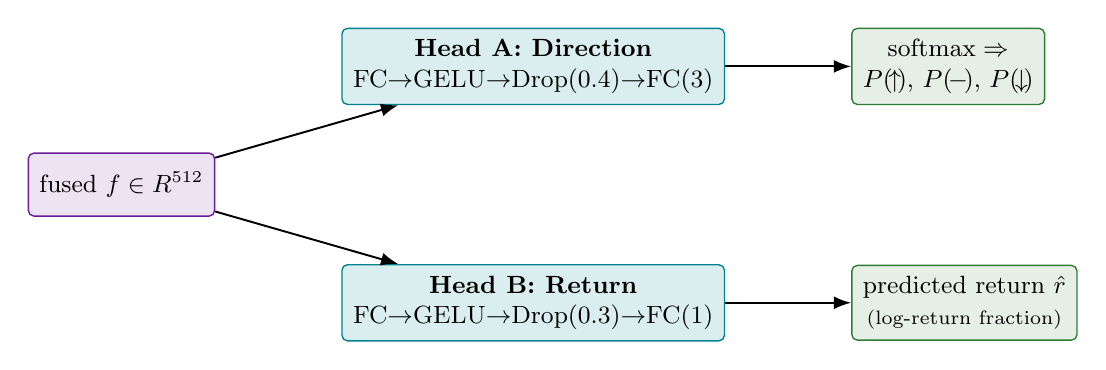
\begin{tikzpicture}[node distance=8mm and 16mm]
\node[fnode] (f) {fused $f\in\mathbb{R}^{512}$};
\node[onode, above right=6mm and 16mm of f] (dch)
   {\textbf{Head A: Direction}\\ FC$\to$GELU$\to$Drop(0.4)$\to$FC(3)};
\node[onode, below right=6mm and 16mm of f] (rch)
   {\textbf{Head B: Return}\\ FC$\to$GELU$\to$Drop(0.3)$\to$FC(1)};
\node[trnode, right=of dch] (probs)
   {$\mathrm{softmax}\Rightarrow$\\ $P(\!\uparrow\!),\,P(\!-\!),\,P(\!\downarrow\!)$};
\node[trnode, right=of rch] (ret) {predicted return $\hat r$\\ \scriptsize (log-return fraction)};

\draw[arr] (f) -- (dch);
\draw[arr] (f) -- (rch);
\draw[arr] (dch) -- (probs);
\draw[arr] (rch) -- (ret);
\end{tikzpicture}}
\caption{Dual-head output: a 3-class direction classifier (calibrated softmax) and a scalar return-magnitude regressor.}
\end{figure}

% =====================================================================
% FIGURE 6 — WGAN-GP CRISIS AUGMENTATION
% =====================================================================
\begin{figure}[p]\centering
\resizebox{0.92\textwidth}{!}{%
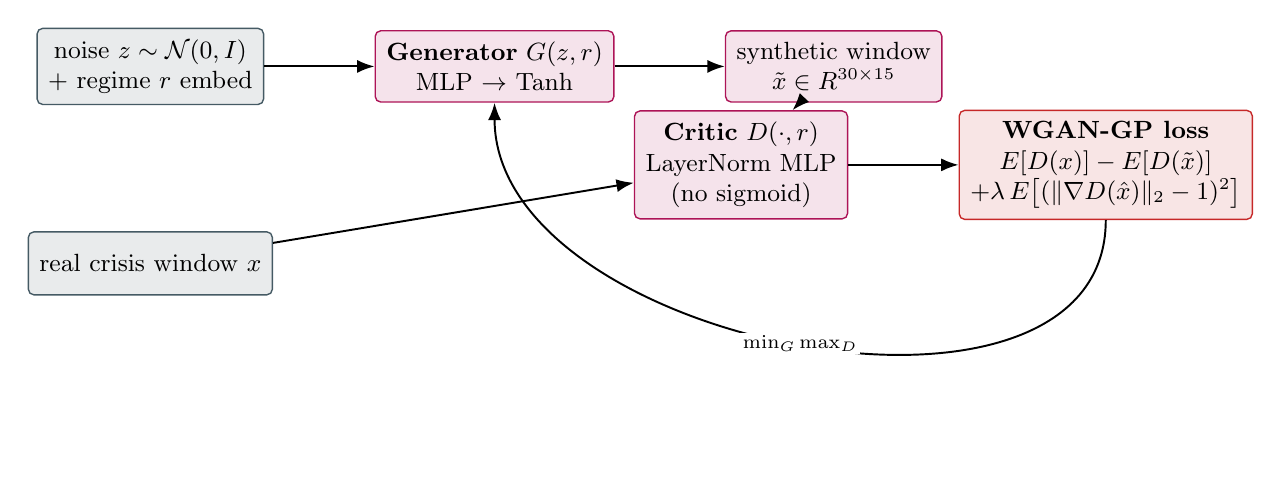
\begin{tikzpicture}[node distance=8mm and 14mm]
\node[io] (z) {noise $z\sim\mathcal{N}(0,I)$\\ $+$ regime $r$ embed};
\node[gnode, right=of z] (G) {\textbf{Generator} $G(z,r)$\\ MLP $\to$ Tanh};
\node[gnode, right=of G] (fake) {synthetic window\\ $\tilde x\in\mathbb{R}^{30\times15}$};
\node[io, below=16mm of z] (real) {real crisis window $x$};

\node[gnode, right=18mm of $(fake)!0.5!(real)$] (C)
   {\textbf{Critic} $D(\cdot,r)$\\ LayerNorm MLP\\ (no sigmoid)};
\node[rnode, right=of C] (loss)
   {\textbf{WGAN-GP loss}\\
    $\mathbb{E}[D(x)]-\mathbb{E}[D(\tilde x)]$\\
    $+\lambda\,\mathbb{E}\big[(\Vert\nabla D(\hat x)\Vert_2-1)^2\big]$};

\draw[arr] (z)--(G); \draw[arr] (G)--(fake);
\draw[arr] (fake) -- (C);
\draw[arr] (real) -- (C);
\draw[arr] (C) -- (loss);
\draw[arr] (loss.south) to[out=-90,in=-90] node[lbl,pos=0.5]{$\min_G\max_D$} (G.south);
\end{tikzpicture}}
\caption{WGAN-GP augmentation: regime-conditioned generator and gradient-penalty critic synthesize rare crisis-regime price windows to harden the model.}
\end{figure}

% =====================================================================
% FIGURE 7 — TRAINING PIPELINE
% =====================================================================
\begin{figure}[p]\centering
\resizebox{\textwidth}{!}{%
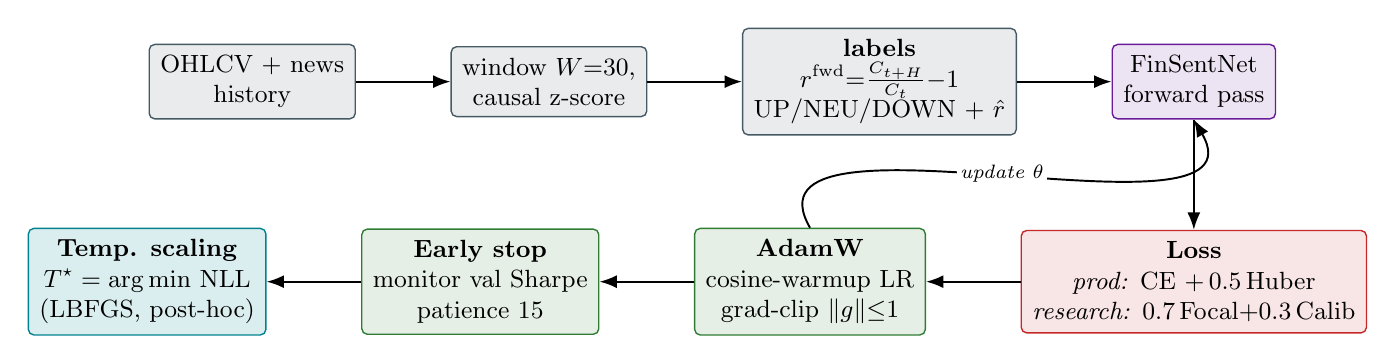
\begin{tikzpicture}[node distance=6mm and 12mm]
\node[io] (data) {OHLCV + news\\ history};
\node[io, right=of data] (win) {window $W{=}30$,\\ causal z-score};
\node[io, right=of win] (lab)
   {\textbf{labels}\\ $r^{\mathrm{fwd}}{=}\tfrac{C_{t+H}}{C_t}{-}1$\\
    UP/NEU/DOWN + $\hat r$};
\node[fnode, right=of lab] (model) {FinSentNet\\ forward pass};

\node[rnode, below=14mm of model] (loss)
   {\textbf{Loss}\\
    \emph{prod:} CE $+\,0.5\,$Huber\\
    \emph{research:} $0.7\,$Focal$+0.3\,$Calib};
\node[trnode, left=of loss] (opt)
   {\textbf{AdamW}\\ cosine-warmup LR\\ grad-clip $\Vert g\Vert{\le}1$};
\node[trnode, left=of opt] (es)
   {\textbf{Early stop}\\ monitor val Sharpe\\ patience 15};
\node[onode, left=of es] (cal)
   {\textbf{Temp. scaling}\\ $T^\star=\arg\min$ NLL\\ (LBFGS, post-hoc)};

\draw[arr] (data)--(win); \draw[arr] (win)--(lab); \draw[arr] (lab)--(model);
\draw[arr] (model)--(loss); \draw[arr] (loss)--(opt); \draw[arr] (opt)--(es);
\draw[arr] (es)--(cal);
\draw[arr] (opt.north) to[out=120,in=-60] node[lbl]{update $\theta$} (model.south);
\end{tikzpicture}}
\caption{Training pipeline: causal windowing/labeling $\to$ multi-task loss $\to$ AdamW + cosine warmup $\to$ early-stop on Sharpe $\to$ post-hoc temperature calibration.}
\end{figure}

% =====================================================================
% FIGURE 8 — INFERENCE -> DECISION -> FINAL SUMMARY
% =====================================================================
\begin{figure}[p]\centering
\resizebox{\textwidth}{!}{%
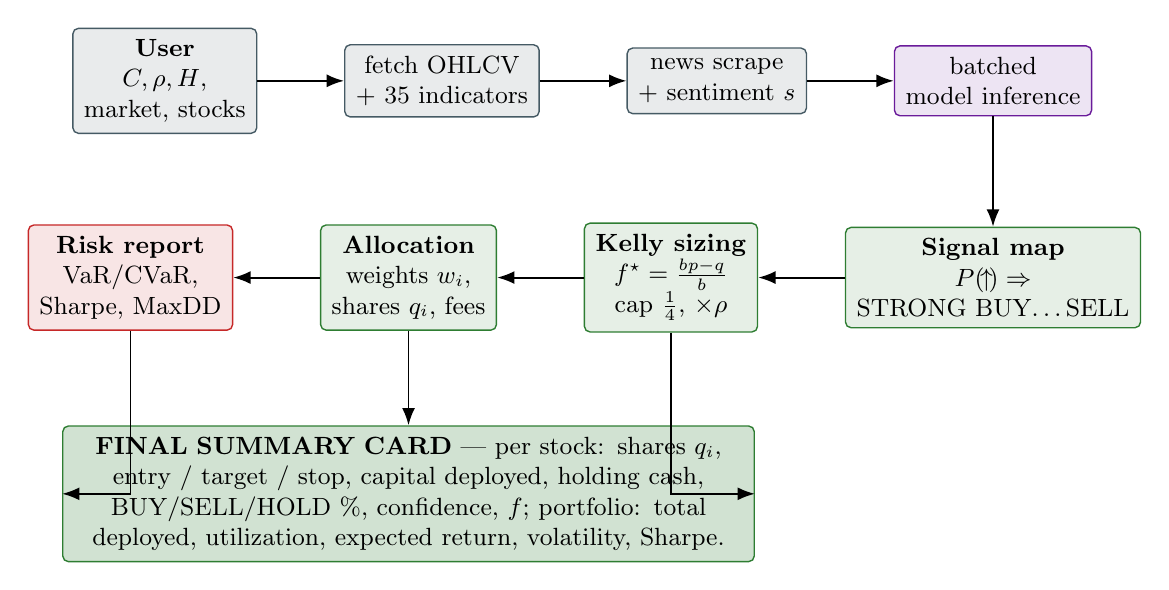
\begin{tikzpicture}[node distance=6mm and 11mm]
\node[io] (u) {\textbf{User}\\ $C,\rho,H$,\\ market, stocks};
\node[io, right=of u] (fetch) {fetch OHLCV\\ + 35 indicators};
\node[io, right=of fetch] (sent) {news scrape\\ + sentiment $s$};
\node[fnode, right=of sent] (infer) {batched\\ model inference};

\node[trnode, below=14mm of infer] (map)
   {\textbf{Signal map}\\ $P(\!\uparrow\!)\Rightarrow$\\ STRONG BUY$\dots$SELL};
\node[trnode, left=of map] (size)
   {\textbf{Kelly sizing}\\ $f^\star=\tfrac{bp-q}{b}$\\ cap $\tfrac14$, $\times\rho$};
\node[trnode, left=of size] (alloc)
   {\textbf{Allocation}\\ weights $w_i$,\\ shares $q_i$, fees};
\node[rnode, left=of alloc] (riskr)
   {\textbf{Risk report}\\ VaR/CVaR,\\ Sharpe, MaxDD};

\node[io, below=12mm of alloc, fill=cTrade!22, draw=cTrade, text width=85mm] (sum)
   {\textbf{FINAL SUMMARY CARD} --- per stock: shares $q_i$, entry / target / stop,
    capital deployed, holding cash, BUY/SELL/HOLD \%, confidence, $f$;
    portfolio: total deployed, utilization, expected return, volatility, Sharpe.};

\draw[arr] (u)--(fetch); \draw[arr] (fetch)--(sent); \draw[arr] (sent)--(infer);
\draw[arr] (infer)--(map); \draw[arr] (map)--(size); \draw[arr] (size)--(alloc);
\draw[arr] (alloc)--(riskr);
\draw[arr] (alloc)--(sum);
\draw[arr] (size.south) |- (sum.east);
\draw[arr] (riskr.south) |- (sum.west);
\end{tikzpicture}}
\caption{Inference-to-decision flow: user selection $\to$ data + sentiment $\to$ model $\to$ discrete signal + Kelly sizing + allocation + risk $\to$ final investment summary.}
\end{figure}

\end{document}
